In this section we will present a general overview of the system-to-be, with a specific focus on the main logical components and their interactions. \\ \\
The main high-level components of the system are:
\subsubsection{Mobile App:}
\label{subsubsect:Mobile App}
The presentation layer that lets the users access the functionalities offered by the Travlendar+ on their smartphones. The mobile application offers also an internal logic that handles:
\begin{itemize}
	\item the notifications reception, through Google Cloud Messaging APIs;
	\item the display of the map and the drawing of the path through Google Maps mobile APIs.
\end{itemize}  

\subsubsection{Web Browser:}
\label{subsubsect:Web Browser}
The presentation layer that lets the users access the functionalities offered by the Travlendar+ on their browsers.
It relies on the connection with the web server in order to obtain dynamic web pages.

\subsubsection{Web Server:}
\label{subsubsect:Web Server}
This layer provides web pages for the web-based application, it communicates directly with the application server interfaces to satisfy the client requests, using proper interfaces. This layer interacts also with an external system (Google Maps API) in order to display an embedded map containing the user travel's information.

\subsubsection{Application Server:}
\label{subsubsect:Application Server}
The logic layer that implements all the functionalities of the core system. It receives and replies to client's requests, if required it sends notifications to the mobile applications, it interacts with external systems in order to satisfy the user's requests and it interacts with a DBMS in order to guarantee the information persistence.
In particular, the application server will interact with:
\begin{itemize}
\item Google Maps APIs, in order to provide feasible paths according to the user preferences;
\item Transport Service providers systems to supply trips arranging functionalities, such as ticket buying, location of sharing vehicles and strikes information;
\item Weather APIs, in order to provide weather information and to apply possible travel constraints related to the weather;
\item Google Cloud Messaging APIs, in order to send notifications to the user's mobile apps.
\end{itemize} 
\subsubsection{Database Server:}
\label{subsubsect:Database Server}
The data layer, that supports all data storage and management operations. This layer ensures that ACID properties are satisfied. The database server will interact only with the application server, so that the data will never be exposed directly to the client layers.
\subsubsection{External Systems:}
\label{subsubsect:External Systems}
Those systems are not internal components of our application, but the system-to-be will have to interact with them in order to guarantee all the system functionalities. \\
Most of their interactions with the system have already been described in the previous paragraphs, but here we will explain in detail the interaction with Transport Service providers: Travlendar+ will initially integrate some external transport services systems (public transport service providers and sharing vehicles provider) but will also offer proper APIs to allow others Transport Service providers to interact with Travlendar+ and therefore to be considered as suggested travel means to the users.


\begin{figure}[H]
\begin{center}
		\hspace*{-50pt}
		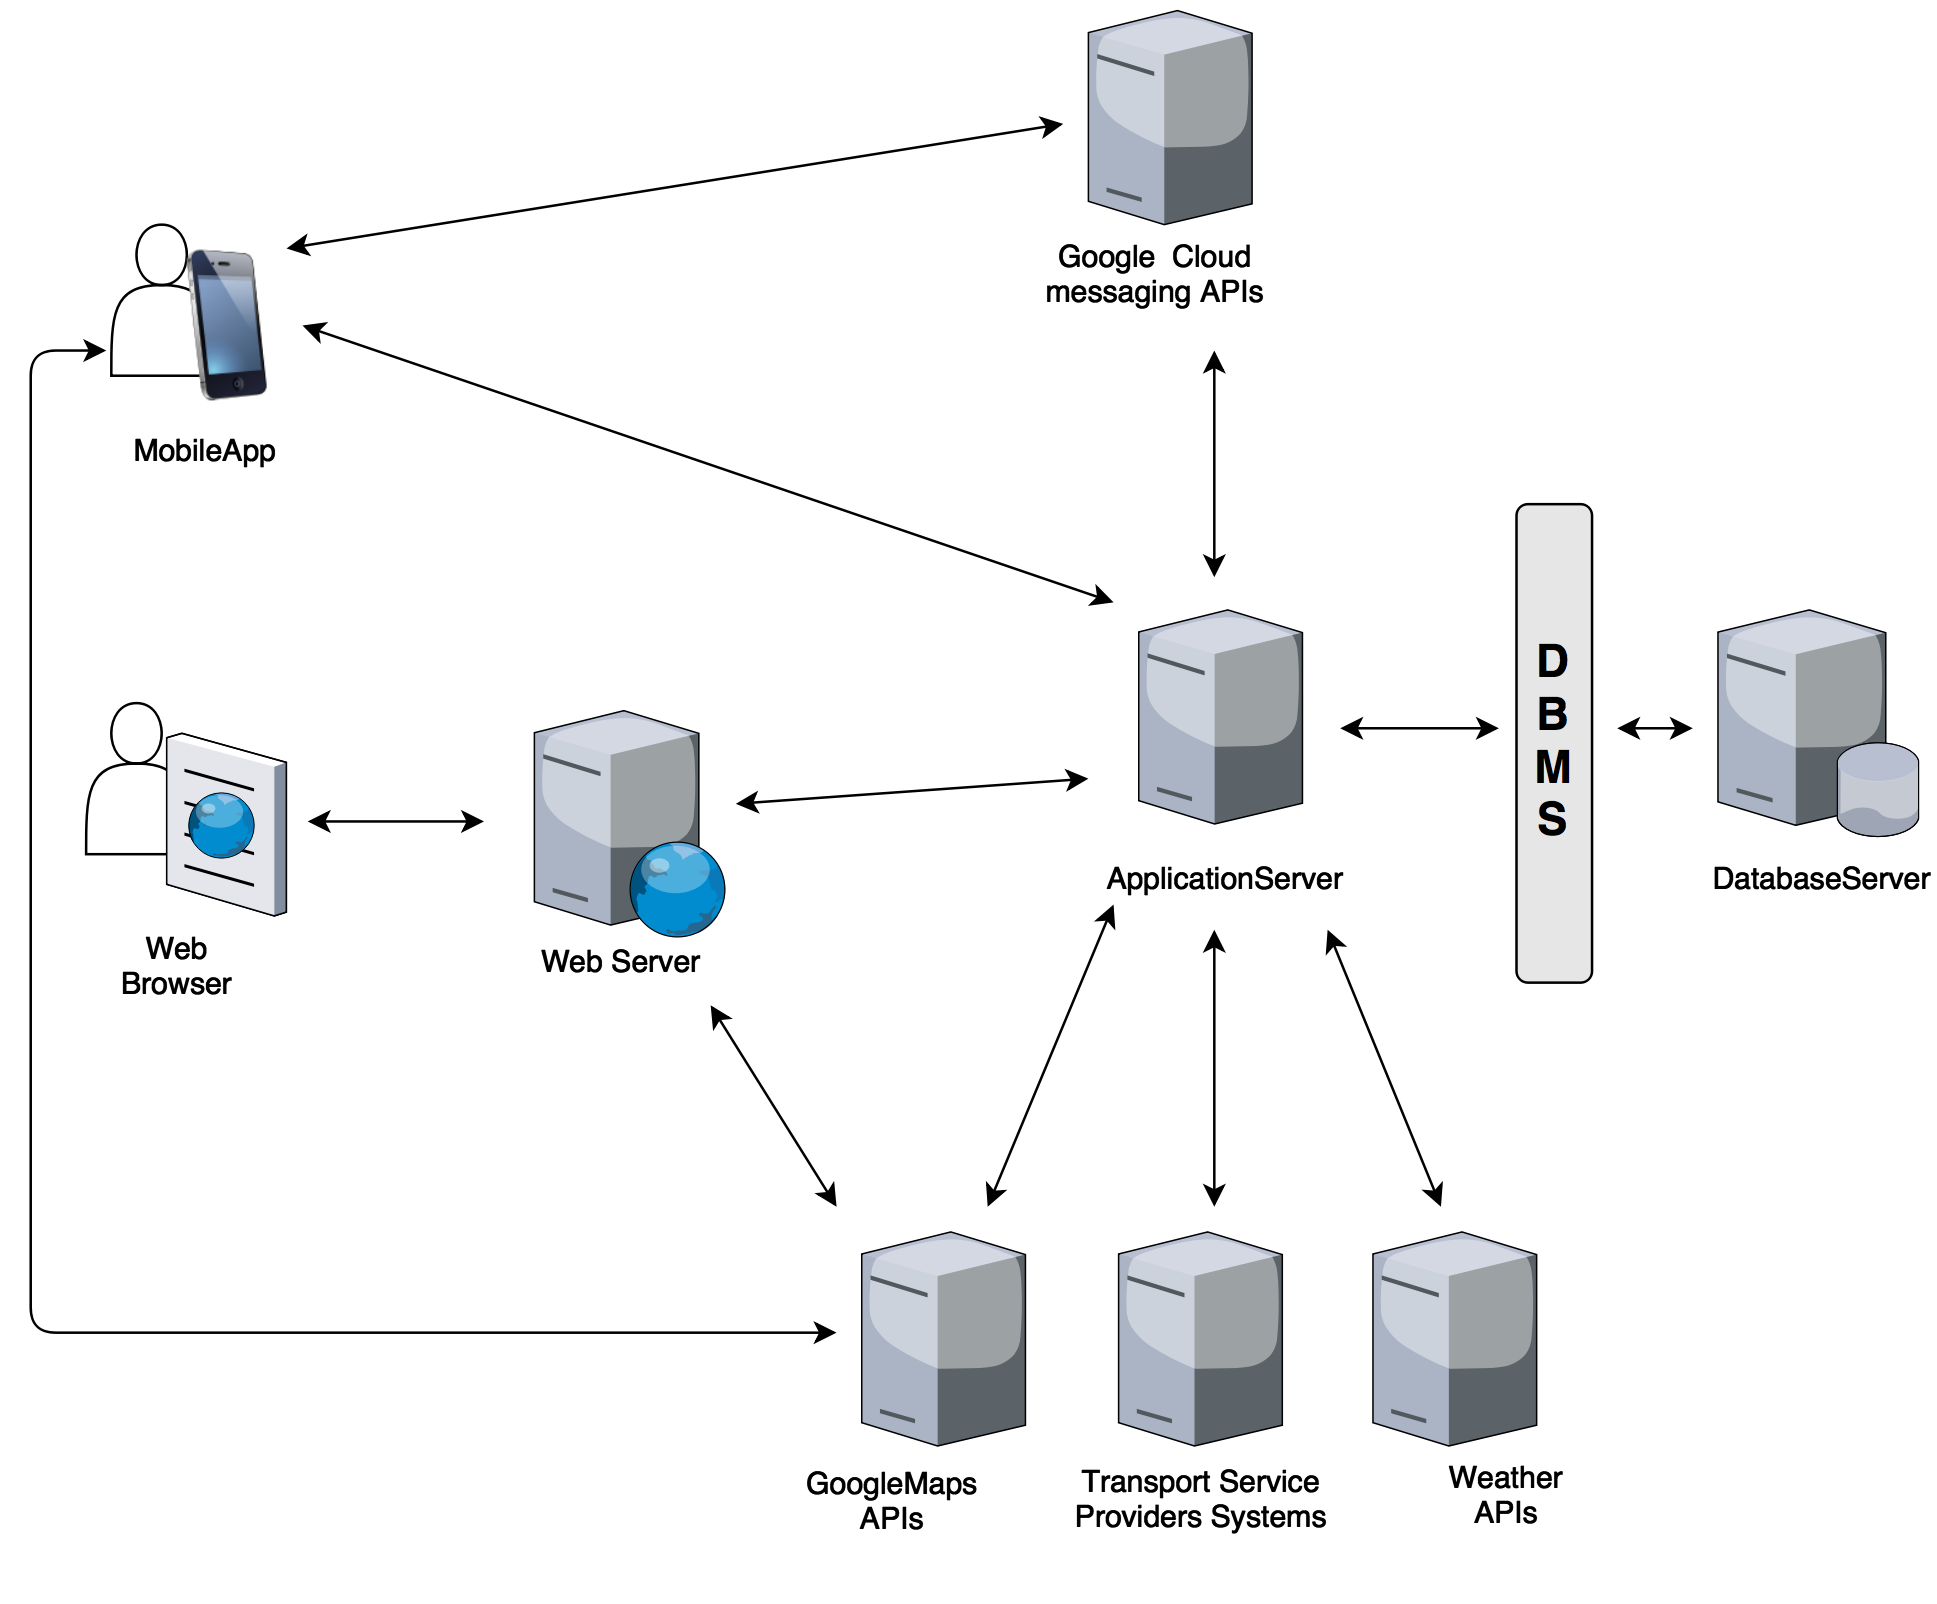
\includegraphics[scale=0.2]{GeneralArchitecture.png}
\end{center}
\caption{General Architecture}
\end{figure}
